\documentclass[12pt]{article}
\usepackage[a4paper]{geometry}
\usepackage{setspace}
\usepackage{graphicx}
\usepackage{lipsum}
\usepackage{fancyhdr}
\usepackage{multicol}

\pagestyle{fancy}
\graphicspath{{images/}}
\setlength{\headheight}{15pt}

\begin{document}

    \begin{titlepage}
    \begin{center}
        \vspace*{1cm}
        
        \Huge
        \textbf{Merencanakan Sebuah Sistem}
        
        \vspace{0.5cm}
        \LARGE
        Bagaimana kemajuan software mengubah cara kita merencanakan dunia

        \vspace{1.5cm}
        
        \textbf{Zainal - Rafli - Sylvano - Vincent - Kal-el}
        
        
        % A thesis presented for the degree of\\
        % Doctor of Philosophy
        
        \vspace{1cm}
        
        
\includegraphics[width=0.6\textwidth]{images/letrisLogo.jpg}
        
        \vfill

        \Large
        Rekayasa Perangkat Lunak\\
        Sekolah Menengah Kejurusan Letris 2\\
        % Indonesia\\
        10 September 2023
        
    \end{center}
\end{titlepage}

    % \chapter*{Abstrak}
    
    \tableofcontents
    
    \newpage
    
    \section{Pendahuluan}
    \thispagestyle{plain}

Abad ke-21 adalah abad yang tiada duanya.\\ \\Di mana revolusi industri 
melahirkan tingkat produktivitas dan pertumbuhan yang belum pernah terjadi pada sejarah peradaban manusia,
menaklukkan alam pada kehendak manusia, yang dapat membuat nenek moyang primata kita menjerit dan meringis
dalam kekaguman dan ketakutan akan kekuatan layaknya seorang dewa. 

Perkembangan ilmu pengetahuan dan teknologi nuklir merupakan puncak dari pengetahuan ilmiah abad ke-20,
umat manusia tidak lagi hanya mampu memanfaatkan kekuatan batu bara dan baja untuk menggerakkan mesin-mesin perkasa,
tetapi fondasi dasar dari alam semesta materi kita sendiri, atom, berada di genggam tangan kita dengan memungkinkannya kekuatan nuklir untuk penggunaan manusia... untuk baik atau tidak.

Tidak ada seorang pun yang dapat menghindari gelombang kemajuan industri modern yang tak tertahankan.
Pada saat itu, anda tentu tidak akan salah jika berpikir bahwa umat manusia telah mencapai klimaks akhir sebagai peradaban.

% Namun, sekarang, manusia abad ke-21 sedang menyaksikan apa yang disebut sebagai
% "revolusi industri keempat". Sebuah istilah yang pertama kali dicetuskan oleh
% ketua \emph{World Economic Forum} Klaus Schwab. Dan kunci baru untuk era ini adalah \textbf{data}, 
% sebuah dunia baru di mana data menggerakkan roda industri, 
% setiap perusahaan mulai dari toko swalayan kecil hingga
% perusahaan teknologi raksasa multi nasional seperti google mengumpulkan data dalam skala 
% yang belum pernah terjadi sebelumnya. Dan memang tidak heran, 
% data yang baik dan beragam dengan analisis yang berpengalaman dan berpengetahuan
% luas dapat membuat perbedaan antara rencana yang menguntungkan dan rencana yang membawa bencana.

% Menurut analysis dari World Economic Forum \cite{WEF}, Setiap hari di Bumi,
% kita menghasilkan 500 juta tweet, 294 miliar email,
% 4 juta gigabyte data Facebook, 65 miliar pesan WhatsApp, 
% dan 720.000 jam konten baru yang ditambahkan setiap hari di YouTube. Pada tahun 2018, 
% jumlah total data yang dibuat, ditangkap, disalin, dan dikonsumsi di dunia adalah 33 zettabyte (ZB) - 
% setara dengan 33 triliun gigabyte. Jumlah ini meningkat menjadi 59 ZB pada tahun 2020 dan diprediksi akan 
% mencapai 175ZB pada tahun 2025. Satu zettabyte adalah 8.000.000.000.000.000.000 bit.

% Untuk membantu memvisualisasikan angka-angka ini, 
% mari kita bayangkan setiap bit adalah koin £1, yang tebalnya sekitar 3mm (0,1 inci).
% Satu ZB yang terdiri dari setumpuk koin akan menjadi 2.550 tahun cahaya. 
% Ini bisa membawa Anda ke sistem bintang terdekat, Alpha Centauri, sebanyak 600 kali.

Karena itu, perkembangan industri modern berada dalam
keadaan yang spesial dibanding pada masa-masa yang lalu. Munculnya
kepentingan software pada pengembangan
sistem informasi. Pengunaan data yang baik sangat penting untuk pengembangan sistem informasi yang
berkualitas, dari \emph{requirement analysis, client feedback, debugging, dll} merupakan fondasi dasar
dari perkembangan sistem informasi modern.

Belum lama ini, Watt S. Humphrey, yang dikenal sebagai bapak kualitas dalam software, mengatakan:
\textbf{"Setiap bisnis adalah bisnis software."}
Baru-baru ini, CEO Microsoft, Satya Nadella, mengulangi kutipan tersebut: 
\textbf{"Setiap perusahaan adalah perusahaan software".}\cite{BMC}
Tentu saja, kita bisa menunjuk ke banyak perusahaan teknologi tertentu yang mengembangkan software.
Jika ada sebuah aplikasi, pasti ada yang mengembangkannya.
Namun organisasi bisnis yang tidak "bergerak di bidang software" mengandalkan perangkat 
lunak dan teknologi untuk menjalankan bisnisnya (dengan kata lain, semuanya). 
Organisasi-organisasi ini perlu mengadaptasi setidaknya beberapa solusi \emph{off-the-shelf}, 
kemungkinan besar akan menyesuaikan software untuk menyelaraskan dan mengoptimalkan dengan 
operasi bisnis mereka yang unik.

Dari kebutuhan akan lebih banyaknya software pada perkembangan semua bidang industri,
muncullah \emph{Systems Development Life Cycle} (SDLC), yang berguna untuk membantu pembuatan software
dengan jaminan kualitas dan ketetapan deadline dengan struktur yang jelas yang memastikan perkembangan
software berjalan sesuai dengan keinginan klien, waktu, dan funding.
    
    \newpage
    
    \begin{multicols}{2}
        \section{Systems Development Life Cycle}
        \subsection{Apa itu SDLC?}
SDLC atau \emph{Systems Development Life Cycle}, atau  
dalam bahasa Indonesia disebut Siklus Hidup Pengembangan Sistem. SDLC adalah siklus yang 
digunakan dalam pembuatan atau pengembangan sistem informasi yang bertujuan untuk menyelesaikan
masalah secara efektif. Dalam pengertian lain, SDLC adalah tahapan kerja yang bertujuan untuk 
menghasilkan sistem berkualitas tinggi yang sesuai dengan keinginan pelanggan atau tujuan dibuatnya
sistem tersebut. SDLC menjadi kerangka yang berisi langkah-langkah yang harus dilakukan untuk 
memproses pengembangan suatu perangkat lunak. Sistem ini berisi rencana lengkap untuk mengembangkan, 
dan memelihara hasil produk software yang jadi.\cite{binus}

\subsection{Fungsi SDLC}
SDLC digunakan untuk membangun suatu sistem informasi agar dapat berjalan sesuai 
dengan apa yang diharapkan. SDLC (Systems Development Life Cycle) 
atau Systems Life Cycle, dalam rekayasa sistem dan rekayasa perangkat lunak, 
adalah proses pembuatan dan pengubahan sistem serta model dan metodologi yang digunakan untuk 
mengembangkan sistem-sistem tersebut. Konsep ini umumnya merujuk pada sistem komputer atau informasi. 
SDLC juga merupakan pola yang diambil untuk mengembangkan sistem perangkat lunak, yang terdiri dari 


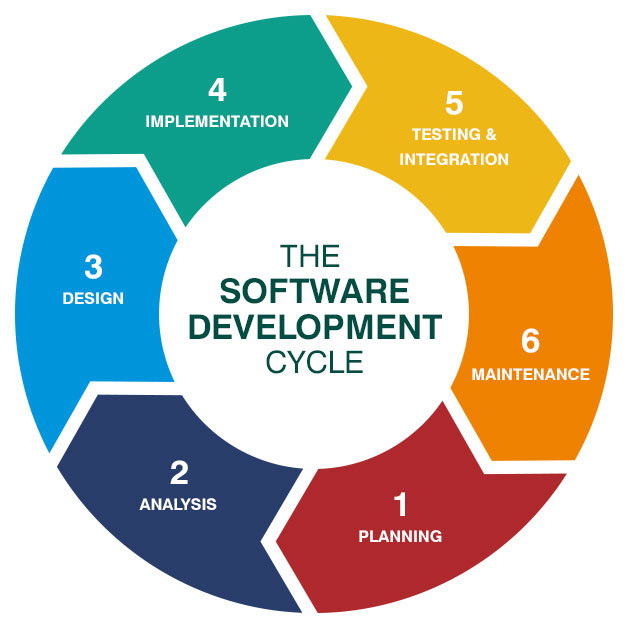
\includegraphics[width=0.4\textwidth]{images/sdlc-cycle.jpg}
tahap-tahap: 


\begin{enumerate}
    \item \emph{Planning} (rencana)
    \item \emph{Analysis} (analysis)
    \item \emph{Design} (design)
    \item \emph{Implementation} (penerapan)
    \item \emph{Testing} (uji coba)
    \item \emph{Maintenance} (pengelolaan)
\end{enumerate}

Dalam rekayasa perangkat lunak, konsep SDLC mendasari berbagai jenis metodologi 
pengembangan perangkat lunak. Metodologi-metodologi ini membentuk suatu kerangka kerja 
untuk perencanaan dan pengendalian pembuatan sistem informasi, yaitu proses pengembangan 
perangkat lunak. Terdapat 3 jenis metode siklus hidup sistem yang paling banyak digunakan, 
yakni: 

\begin{itemize}
    \item \emph{Traditional System Life Cycle}
    \item \emph{Life Cycle Using Prototyping}
    \item \emph{Object-oriented System Life Cycle}
\end{itemize}
    
        \section{SDLC Type Baru}
        \lipsum[1-5]


        
        \section{Pendahuluan}
        \lipsum[1-5]
    
        \section{Pendahuluan}
        
\lipsum[1-5]
        
        \section{Pendahuluan}
        \lipsum[1-5]


        
        \section{Pendahuluan}
        
\lipsum[1-5]


    \end{multicols}
    
\end{document}